\chapter{Outlook and Conclusion}\label{ch:conclusion}

\section{Outlook}

An example to use word embeddings for more advanced tasks is text classification. 
The idea is to map a collection of words given by a text to an image:

\begin{enumerate}
  \item 
    Imagine the following word vectors obtained by GloVe:
    \[
    \begin{array}{c|ccc}
      A & 0.1 & 0.2 & 0.1 \\
      B & 0.2 & 0.5 & 0.3 \\
      C & 0.9 & 0.7 & 0.3 \\
      D & 0.4 & 0.8 & 0.1
    \end{array} \ \ \Rightarrow \ \ w_i \in \mathbb{R}^3, \ d = 3
    \]
    Note that word vectors created by GloVe are organized as rows within the matrix
    where the rownames displays the vocabulary of available words.

  \item 
     Now we have a given text:
    \[
    \mathrm{A\ B\ A\ D\ B\ C}
    \]    

  \item  
    Next, each word in the text is mapped to the corresponding
    word vector to obtain a matrix for the given text:
    \[
    \begin{array}{cccccc}
    \mathrm{A} & \mathrm{B} & \mathrm{A} & \mathrm{D} & \mathrm{B} & \mathrm{C} \\
    \downarrow & \downarrow & \downarrow & \downarrow & \downarrow & \downarrow \\
    0.1 & 0.2 & 0.1 & 0.4 & 0.2 & 0.9 \\
    0.2 & 0.5 & 0.2 & 0.8 & 0.5 & 0.7 \\
    0.1 & 0.3 & 0.1 & 0.1 & 0.3 & 0.3
    \end{array}
    \]
  
  \item 
    This matrix can be used to create an image out of the 
    given text by translating the matrix to an image:

\begin{figure}[!h]
\centering
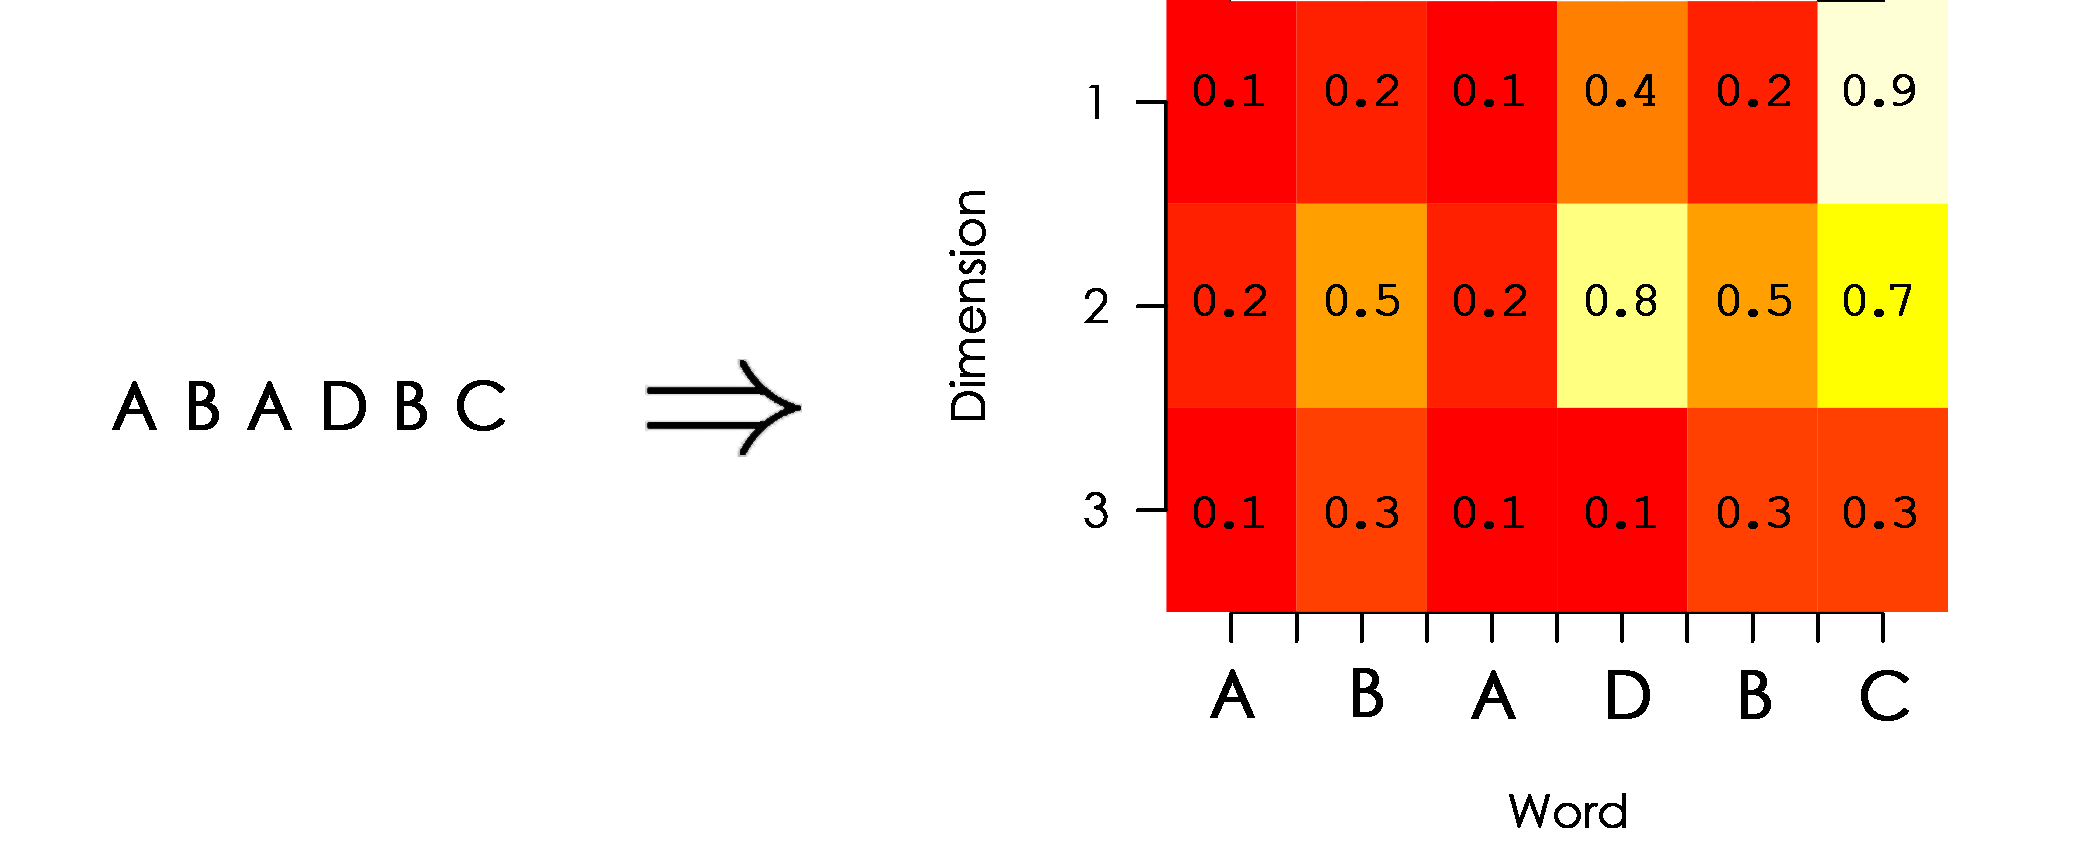
\includegraphics[width=0.7\textwidth]{images/image_classif.png} 
\caption[Example of the text to image procedure.]{Explanation of the mapping 
         between text and image.}
\label{fig:text-classif}
\end{figure}
\end{enumerate}

The images in figure \ref{fig:text-classif-images} were generated from the
introduction of Principia Mathematica by Sir Isaac Newton and Elements of 
Statistical Learning, as well as from Sonnet 18 by William Shakespear. \\

\begin{figure}[!h]
\centering

\includegraphics[width=\textwidth]{images/text_images.png} 
\caption[Specific text representation via images.]{Creating images for text using 
         the introduction of Principia Mathematica by Sir Isaac Newton and 
         Elements of Statistical Learning, as well as from Sonnet 18 by William 
         Shakespear. The red bars are missing words filled up to 150 words since 
         image classifier expect a fixed number of pixels.}
\label{fig:text-classif-images}
\end{figure}

The next step would be to run an image classifier (e.~g.~a CNN) on the images
and an label. This classifier could find differences by analysing specific patterns
or maybe the color intensity.

\section{Conclusion}

The aim of GloVe was to create meaningful word embeddings. After evaluating the created word vectors
this is definitely the case. The word vectors are able to catch word similarities as well as
semantic analogies between words by keeping the linear structure of the word vector space. What hasn't 
been mentioned so far is that Pennington et al. compare different word embeddings like singular value decomposition (SVD) or CBOW 
which uses neural nets to find the embedding. Table \ref{tab:comparison} shows how the different embeddings
perform on the word similarity task. \\

\begin{table}[!h]
\centering
\begin{tabular}{@{}llllll@{}}
\hline
\textbf{Model} & \textbf{Dim.} & \textbf{Size} & \textbf{Sem.} & \textbf{Syn.} & \textbf{Tot.}\\
\hline\hline
ivLBL & 100 & 1.5B & 55.9 & 50.1 & 53.2\\
HPCA & 100 & 1.6B & 4.2 & 16.4 & 10.8\\
GloVe & 100 & 1.6B & \underline{67.5} & \underline{54.3} & \underline{60.3}\\
\hline
SG & 300 & 1B & 61 & 61 & 61\\
CBOW & 300 & 1.6B & 16.1 & 52.6 & 36.1\\
vLBL & 300 & 1.5B & 54.2 & \underline{64.8} & 60.0\\
ivLBL & 300 & 1.5B & 65.2 & 63.0 & 64.0\\
GloVe & 300 & 1.6B & \underline{80.8} & 61.5 & \underline{70.3}\\
\hline
SVD & 300 & 6B & 6.3 & 8.1 & 7.3\\
SVD-S & 300 & 6B & 36.7 & 46.6 & 42.1\\
SVD-L & 300 & 6B & 56.6 & 63.0 & 60.1\\
CBOW & 300 & 6B & 63.6 & \underline{67.4} & 65.7\\
SG & 300 & 6B & 73.0 & 66.0 & 69.1\\
GloVe & 300 & 6B & \underline{77.4} & 67.0 & \underline{71.7}\\
\hline
CBOW & 1000 & 6B & 57.3 & 68.9 & 63.7\\
SG & 1000 & 6B & 66.1 & 65.1 & 65.6\\
SVD-L & 300 & 42B & 38.4 & 58.2 & 49.2\\
GloVe & 300 & 42B & \underline{\textbf{81.9}} & \underline{\textbf{69.3}} & \underline{\textbf{75.0}}\\
\hline
\end{tabular}
\caption{Comparison of different word embeddings on different corpora (copied from \cite{pennington2014glove}).}
\label{tab:comparison}
\end{table}


Nevertheless, we have also seen that the quality of the word vectors does not only depend on the dimension, but
also on the corpus. Having a good corpus implies that a huge amount of data (maybe some giga or terabytes) has
to be analysed. This isn't possible on normal computers or working stations. Hence, to build own good word vectors
it is indispensable to have access to enormous computing power. The alternative is to take pre trained word 
vectors (e.~g.~provided by Pennington et al.).
%
%  \item 
%    Use servers or pcs with huge computing power to train GloVe due to 
%    the need of huge corpora an computing time!
%\end{itemize}